\documentclass[11pt]{article}
\usepackage[czech]{babel}
\usepackage[T1]{fontenc}
\usepackage[utf8]{inputenc}
\usepackage{graphicx}
\usepackage{epstopdf}
\usepackage[pdfborder=0 0 0]{hyperref}
%% \usepackage{a4wide}

\newcommand\CARET{\mathbin{\char`\^}}


\title{Vizualizace grafu matematické funkce}
\author{Tomáš Maršálek}
\date{\today}

\begin{document}

\begin{titlepage}
\begin{center}
	
\includegraphics{res/znak_vzor.png} \\[2cm]
	\huge{Vizualizace grafu matematické funkce} \\[.2cm]
	\Large{Semestrální práce z předmětu KIV/PC} \\[2cm]
	\Large{Tomáš Maršálek} \\
	\large{marsalet@students.zcu.cz} \\[1cm]
	\normalsize{\today}
\end{center}
\end{titlepage}

\section{Zadání}
Naprogramujte v ANSI C přenositelnou konzolovou aplikaci, která jako vstup
načte z parametru na příkazové řádce matematickou funkci ve tvaru $y = f(x)$,
provede její analýzu a vytvoří soubor ve formátu PostScript s grafem této
funkce na zvoleném definičním oboru.

Kompletní zadání:
\url{http://www.kiv.zcu.cz/studies/predmety/pc/doc/work/sw2011-02.pdf}.

\section{Analýza úlohy}
Abychom mohli zobrazit graf funkce, jako například $f(x) = x * 2 + \sin(x)$,
musíme být nejdříve schopni vyhodnotit tuto funkci numericky. Tedy pro
jakékoliv x chceme redukovat výraz na číslo $y = f(x)$. Vyhodnocování je vhodné
rozdělit do více fází, protože většina práce spočívá v nalezení chyb ve výrazu.
Každá z fází se slouží, kromě svého hlavního účelu, jako filtr pro případné
chyby, které by způsobovaly zbytečné nepříjemnosti ve fázi nadcházející, ta
poté může předpokládat vstupní řetězec bez chyb. 

\subsection{Lexikální analýza}
Místo abychom při vyhodnocování výrazu postupně hledali čísla nebo operátory,
ponecháme tuto úlohu specializovanému nástroji, takzvanému scanneru nebo také
lexeru. Nadefinujeme jednotlivé symboly a necháme scanner, aby je ve vstupním
řetězci rozpoznal nebo aby případně rozpoznal lexikální chyby.  Význam celé
této fáze je ve zjednodušení nadcházející fáze, která je složitější, a už se
nebude muset zabývat problémy typu jestli je symbol skutečně číslo nebo zda
symbol \uv{sin} je ve skutečnosti \uv{sinh} a podobně.

\subsection{Syntaktická a sémantická analýza}
Tyto dvě fáze jsou zde zkombinované v jednu. Vytvoříme přeloženou datovou
strukturu, se kterou bude vyhodnocování výrazu víceméně triviální. Syntaktická
analýza najde chyby týkající se skladby výrazu, jako například dvě čísla nebo
znaky následující po sobě, chybějící závorky a podobně. Jednotlivým symbolům
přiřadíme jejich význam, tj. číslům jejich numerickou hodnotu a operátorům
jejich příslušnou unární nebo binární funkci. 

\subsection{Postfixová notace}
Výsledná datová struktura je posloupnost symbolů v postfixové nebo také
reverzní polské notaci. Výhoda tohoto zápisu oproti klasické infixové notaci
je absence závorek a jednoduchost vyhodnocení výrazu. Při vyhodnocování totiž
vždy, když narazíme na operátor, máme jistotu, že všechny předcházející znaky, 
které operátor vyžaduje, jsou čísla.

Příklad infixové a postfixové notace.
\begin{center}
\begin{tabular}{|l|l|}
\hline
infix & postfix \\
\hline
1 + 1 & 1 1 + \\
1 + 2 * 3 & 1 2 3 * + \\
(1 + 2) * 3 & 1 2 + 3 * \\
x * $\sin$ (x $\CARET$ 2) & x x 2 $\CARET$ $\sin$ * \\
1 - 2 - 3 + 4 $\CARET$ 5 $\CARET$ 6 & 1 2 - 3 - 4 5 6 $\CARET$ $\CARET$ + \\
\hline
\end{tabular}
\end{center}

Metoda na převedení infixového do postfixového zápisu je např. Dijkstrův
Shunting yard algoritmus\cite{wikiShunting}\cite{shewchuk}, který je
standardním postupem díky své jednoduchosti~a výpočetní nenáročnosti. Používají
ho kapesní kalkulátory~i software určený pro jednoduché výpočty kvůli minimální
náročnosti na paměť.



\subsection{Zobrazení grafu}
Jednoduchým řešením, jak zobrazit funkci je vyhodnotit vždy dva sousední body~a
spojit je úsečkou. Důležité je pouze zvolit dostatečně detailní rozdělení osy
x, aby graf nebyl kostrbatý.

Úsporná metoda, která řeší hladkost grafu zobrazené funkce je adaptivní
vyhlazování. Šetření zobrazenými přímkami oceníme zejména u jednoduchých
funkcí, protože rozhodně nepotřebujeme, aby graf funkce $f(x) = x$ byl stejně
detailní jako graf funkce $f(x) = sin(1/x)$, který je kolem nuly velmi
zhuštěný. Taktika je poměrně jednoduchá. Mějme zvolené nějaké počáteční
rozdělení osy x, a pokud při zobrazování jednotlivých úseček zjistíme, že by
došlo k příliš velkému skoku ve sklonu dvou sousedních úseček (výpočetně by
druhá derivace přesahovala jistý zvolený práh), rozdělíme interval mezi $x_i$
a $x_{i + 1}$ na polovinu. Samozřejmě musíme mít nějaký limit tohoto půlení,
protože u funkcí typu $f(x) = sin(1/x)$ by došlo kolem nuly k nekonečnému
půlení. Stejným výpočtem se snažíme zajistit co nejdelší interval, aby nedošlo
ke zbytečnému plýtvání. 

Rozdělení osy x je o poznání hustší, pokud je graf v tomto místě detailnější,
jak je vidět v porovnání dvou různých funkcí.

\begin{figure}[ht!]
\centering
	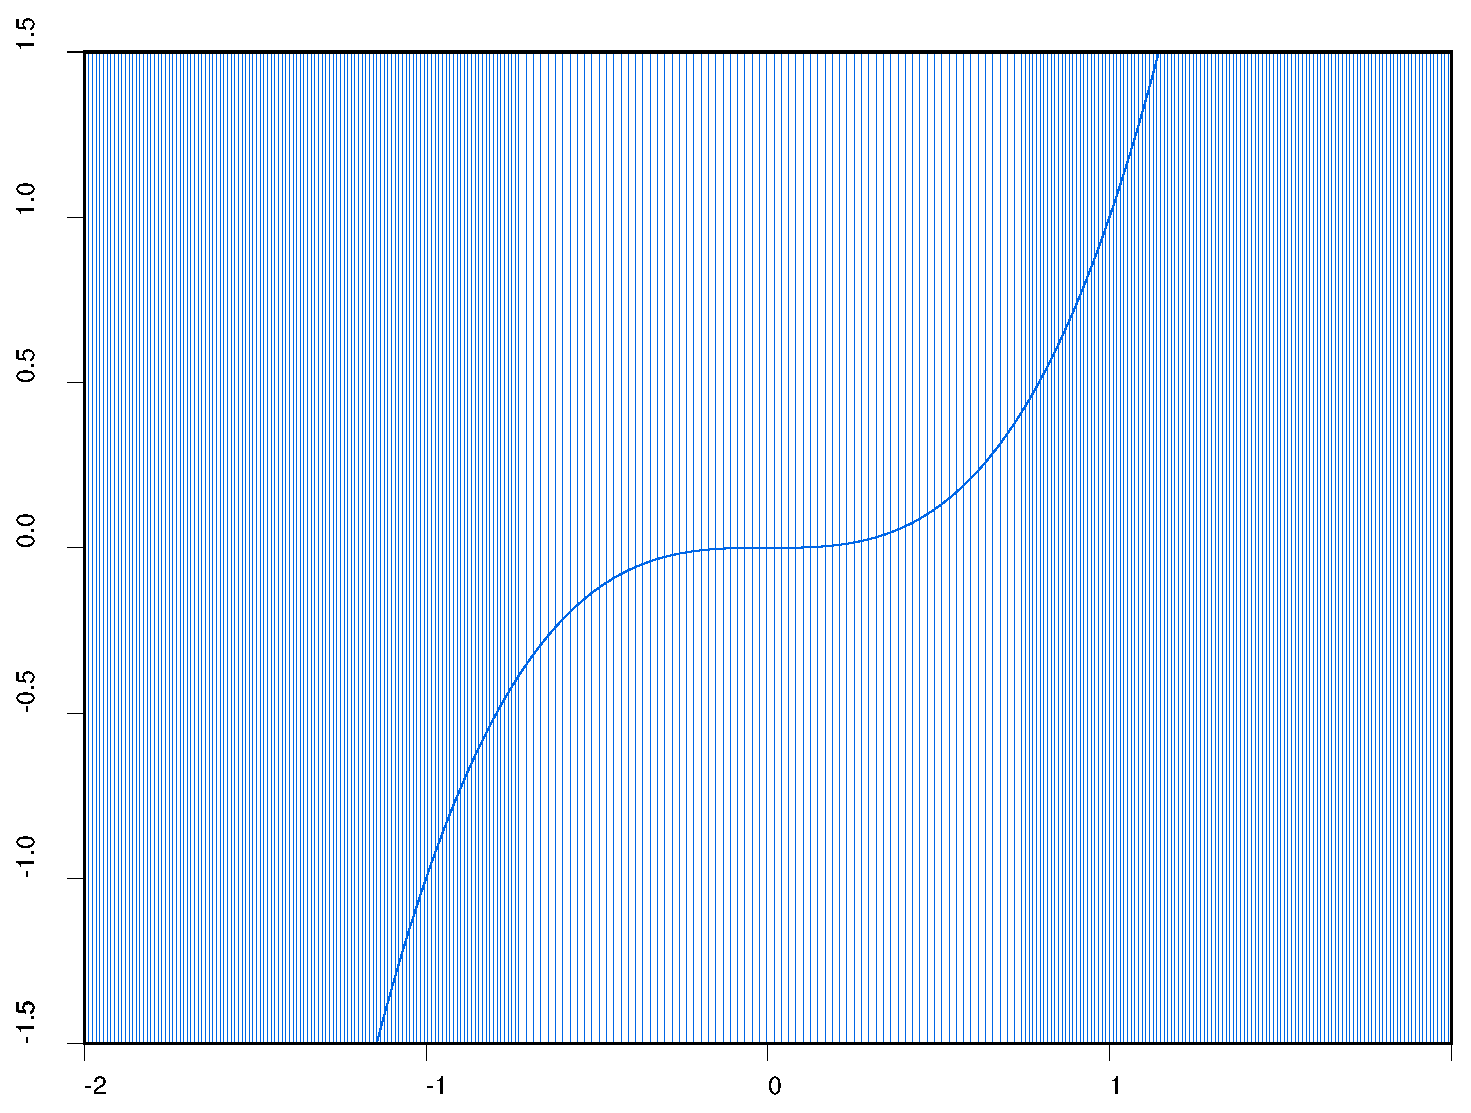
\includegraphics[width=11cm]{figures/figure2.eps}
	\caption{Rozdělení osy x grafu funkce $x^3$}
\end{figure}
\begin{figure}[ht!]
\centering
	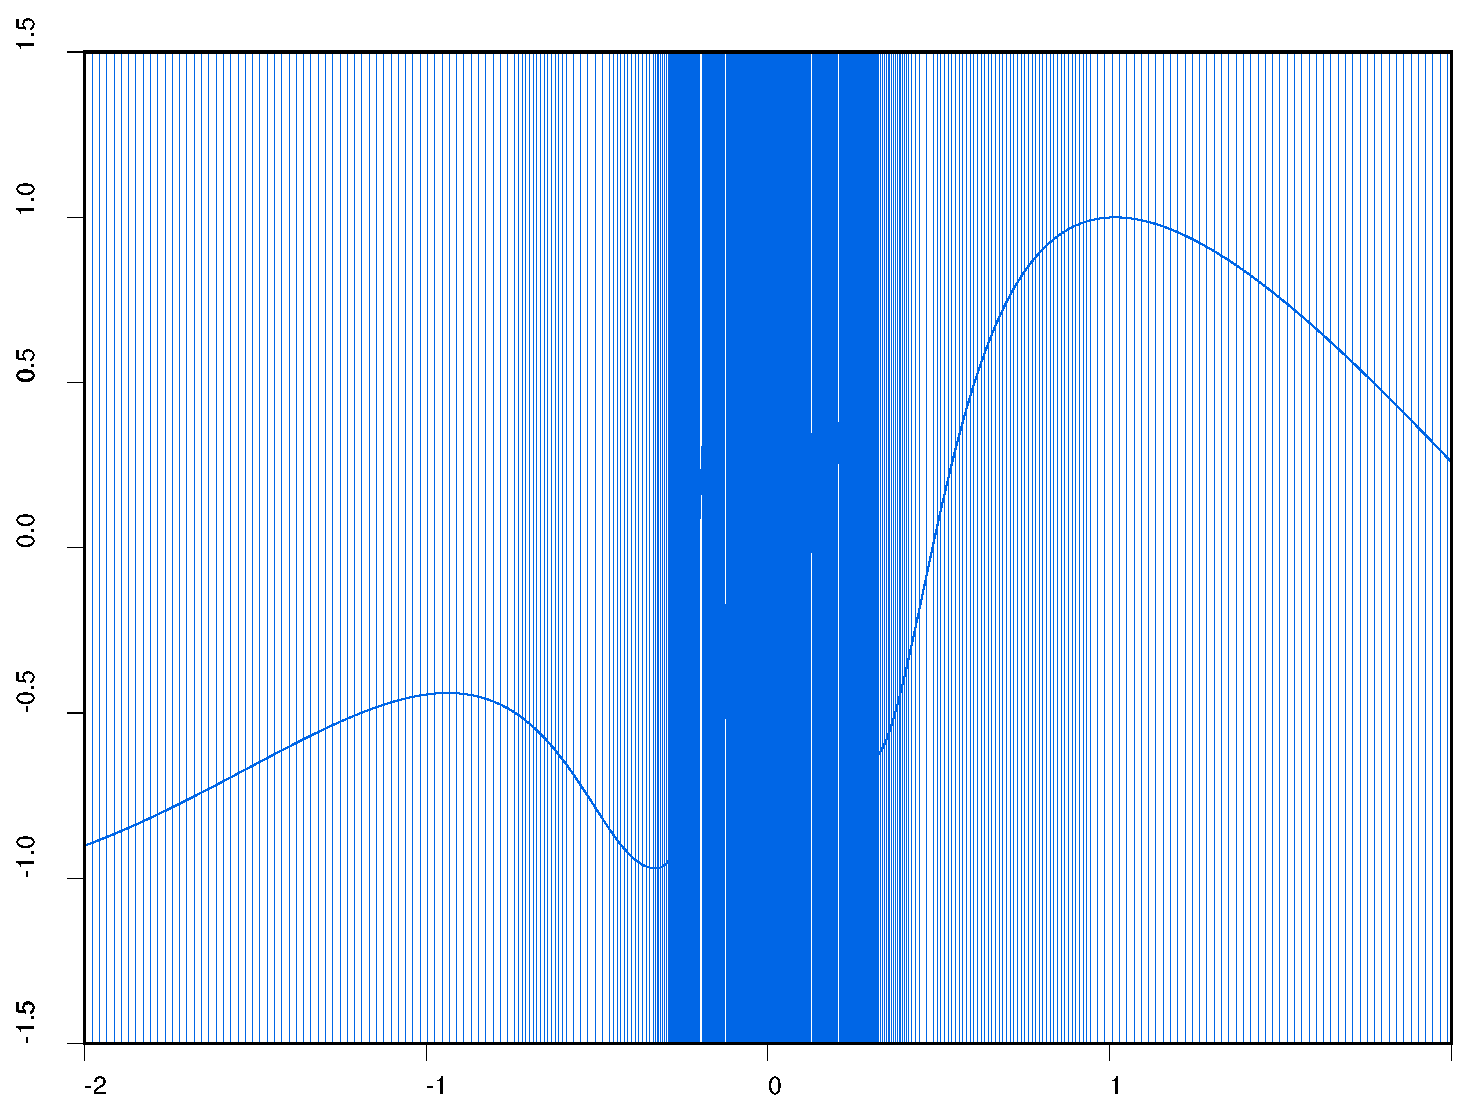
\includegraphics[width=11cm]{figures/figure1.eps}
	\caption{Rozdělení osy x grafu funkce
		$\sin \left(x + \cos \left(\frac{1}{x} \right) \right)$}
\end{figure}

\clearpage
Zřejmým problémem jsou funkce, které v některých bodech zadaného intervalu
rostou limitně do nekonečna, případně nejsou na daném intervalu definovány.
Případ, kdy funkce pokračuje mimo zadanou hranici, případně až do nekonečna, je
celkem jednoduchý. Aby nedošlo k useknutí grafu poblíž dolní nebo horní
hranice, stačí vypočítat průsečík horní nebo dolní hranice s úsečkou mezi
posledním bodem a bodem, který už by byl mimo graf a vést kratší úsečku do
tohoto průsečíku. 
\begin{figure}[ht!]
\centering
	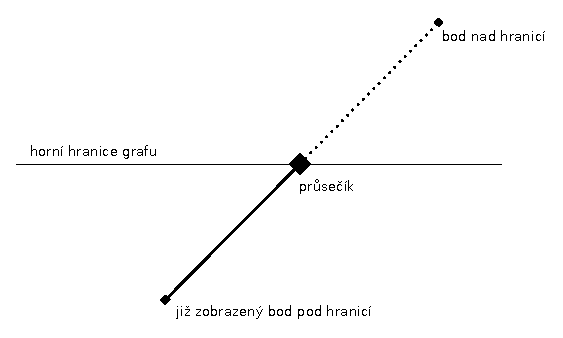
\includegraphics[width=11cm]{figures/boundary.eps}
	\caption{Zamezení úniku grafu mimo hranice}
\end{figure}

Horší jsou funkce, které nejsou definovány v určitém místě. V některých
případech dochází k nežádoucímu vynechání počáteční nebo konečné části grafu.
Příkladem je jakýkoliv logaritmus. Při rozdělení osy x, které vynechá bod $x =
0.0$ dojde k vynechání první úsečky. Ta pak vzhledem k velkému sklonu logaritmu
v tomto místě viditelně schází. Implementace funkcí s nenadefinovanými úseky v
matematické knihovně v takových případech vracejí hodnotu NaN. Výpočet
průsečíku s takovým číslem nedává smysl a předefinování knihovních funkcí na
vlastní, které by vracely alespoň nekonečna namísto NaN způsobuje jiné
nežádoucí artefakty. Například předefinování logaritmů pro záporné hodnoty na
záporné nekonečno funguje, dokud nezobrazíme nějakou transformaci tohoto
logaritmu na reálné hodnoty (např. $f(x) = \exp(\ln(x))$). Pro jednoduchost je
tedy možná lepší NaN hodnoty pouze nezobrazovat.


\section{Implementace}
\subsection{Lexer} 
V souboru \texttt{lexer.c} je konstruován jako deterministický automat, který
rozpoznává celá čísla v šestnáctkové, desítkové a osmičkové soustavě, floating
point čísla, proměnnou x, operátory a závorky. Mezery jsou zahozeny parserem. V
případě chyby posílá chybový token do další fáze.  Token je zde struktura,
která si uchovává pozici a délku nalezeného podřetězce a samotný řetězec pro
případný výpis chyby.

\subsection{Parser}
je implementace Shunting yard algoritmu, která navíc kontroluje syntaktické
chyby. Výsledek je vrácen jako posloupnost symbolů, které ale musí být po
skončení používání dealokovány. Pro zjednoduššení jsou všechny tokeny a
přeložené symboly uchovány v pomocných polích, aby na konci došlo k jejich
bezchybnému dealokování. Symbol je výsledný přeložený token, který je zde
implementován jako polymorfní struktura (uchovává si svůj typ a případně data
vztahující se k jednotlivým typům). Mohla by být implementována i efektivněji,
například pomocí $union$, ale v ANSI C není podporován anonymní $union$. S
pojmenovaným by zdrojový kód vypadal poněkud těžkopádně a navíc k příliš
velkému ušetření paměti by rozhodně nedošlo. Zvolil jsem tedy raději čitelnost
kódu. 

Pomocnou datovou strukturu zde tvoří pouze zásobník, který se využívá při
Shunting yard algoritmu a poté při kontrolním průchodu výsledným postfixovým
výrazem, kdy se potvrdí, že výraz bude skutečně možné vyhodnotit. Zde se
odstraní chyby související s n-aritou operátorů.

Parser se nachází v souboru \texttt{parser.c} a používá pomocný modul
\texttt{func.c}, který se převážně stará o správné definice a správné přiřazení
matematických funkcí symbolům.

\subsection{Shunting yard}
Při konverzi do postfixu musíme mít na paměti přednosti jednotlivých operátorů.
Výraz $1 + 2 * 3$ se musí přeložit jako $1~2~3~*~+$ a ne jako $1~2~+~3~*$.
Dále také musíme myslet na levou nebo pravou asociaci nekomutativních
operátorů, pokud ve výrazů chybí závorky.  Například operátor odčítání
upřednostňuje levé uzávorkování ($1
- 2 - 3 = ((1 - 2) - 3)$) oproti umocňování, které naopak upřednostňuje
  uzávorkování zprava ($2~\CARET~3~\CARET~4 = (2~\CARET~(3~\CARET~4)) =
2^{3^4}$).

Algoritmus používá pomocný zásobník na odkládání operátorů, dokud nemá jistotu
o jejich správném umístění v postfixu. Čteme infixový výraz zleva doprava po
jednotlivých symbolech a vždy, když narazíme na symbol typu číslo nebo proměnná,
pouze ho uložíme do výsledné výstupní fronty. Pokud narazíme na operátor,
všechny operátory, které dosud leží nahoře v zásobníku a vážou se těsněji (mají
vyšší precedenci) než právě vytažený symbol, můžeme přidat do výsledné fronty.
Právě vytažený symbol pak pouze vložíme na zásobník. Až nám dojdou všechny
symboly, pouze vytáhneme všechny operátory ze zásobníku a v tomto pořadí je
přidáme do výsledné fronty. \\

Jako příklad použijme výraz 1 / 2~$\CARET$~3 + 4.
\begin{center}
\begin{tabular}{|c|l|l|r|}
\hline
symbol & výsledek & zásobník & akce \\
\hline
1 & 1 & & číslo, pouze přidáme do fronty \\
/ & 1 & / & dosud žádný operátor v zásobníku\\
2 & 1 2 & / & číslo, pouze přidáme do fronty \\
$\CARET$ & 1 2 & / $\CARET$ & / má slabší vazbu než $\CARET$, necháme být \\
3 & 1 2 3 & / $\CARET$ & číslo, pouze přidáme do fronty \\
+ & 1 2 3 $\CARET$ / & + & $\CARET$ a / mají silnější vazbu než + \\
4 & 1 2 3 $\CARET$ / 4 & + & číslo, pouze přidáme do fronty \\
konec  & 1 2 3 $\CARET$ / 4 + & & konec, přidáme všechny operátory \\

\hline
\end{tabular}
\end{center}

\subsection{Zobrazení grafu}
je zajištěno dalším odděleným modulem \texttt{plot.c}. Ten nejprve zkonstruuje
hlavičku PostScriptového souboru podle specifikace PostScriptu. 

Poté je funkce vyhodnocena v klíčových bodech, které jsou následně
transformovány na souřadnice PostScriptového formátu stránky a spojeny úsečkami
tak, jak bylo popsáno v analýze úlohy. 

Dalším krokem je vytvoření rámečku grafu a pro přehlednost rozdělení obou os.
Velikost jednotlivých dílků je vybrána tak, aby rozdělení osy nebylo příliš
husté ani řídké, a podle konvence, že dílky mají velikost pouze 1, 2 nebo 5
krát mocnina deseti.

Nakonec jsou zapsány závěrečné PostScriptové příkazy a soubor je uzavřen.

Volitelný parametr popisující defiční obor a obor hodnot je analyzován stejným
lexerem, ale má vlastní parsovací funkci.

\section{Uživatelská příručka}
Překlad ze zdrojových kódů provedeme pomocí příkazu \texttt{make} v kořenovém
adresáři pro překlad pomocí \texttt{gcc}. Program spustíme příkazem ./graph.exe
s parametry funkce, výstupní soubor a volitelně rozsah osy x a y, jak je
naznačeno v~usage stringu programu:
\begin{verbatim}
usage: graph.exe FUNCTION FILE [LIMITS]
\end{verbatim}

Aritmetický výraz může obsahovat běžné binární operátory (+,~-,~*,~/,~$\CARET$)
jednoduché závorky \uv{()}, proměnnou \uv{x}, a funkce, které jsou
implementované (jen pod jiným názvem) v knihovně math.h (abs, exp, ln, log,
sin, cos, tan, asin, acos, atan, sinh, cosh, tanh). Konstanty můžou být zadány
jako celá čísla v osmičkové, desítkové nebo šestnáctkové soustavě, nebo jako
floating point čísla v desítkové soustavě (tak jak jsou rozpoznány jazykem~C).

Vygenerovaný graf je soubor typu encapsulated PostScript (.eps) verze~3, může
být použit přímo v typografickém nástroji \LaTeX.

\clearpage
\subsection{Příklady použití}
\begin{verbatim}
./graph.exe "sin(x + 1/x^3) * -x" vystup.ps 
\end{verbatim}
Do souboru vystup.ps je zapsán graf funkce $\sin (1 / x^2)$
s vestavěným definičním oborem a oborem hodnot $x, y \in [-10, 10]$.
\begin{figure}[ht!]
\centering
	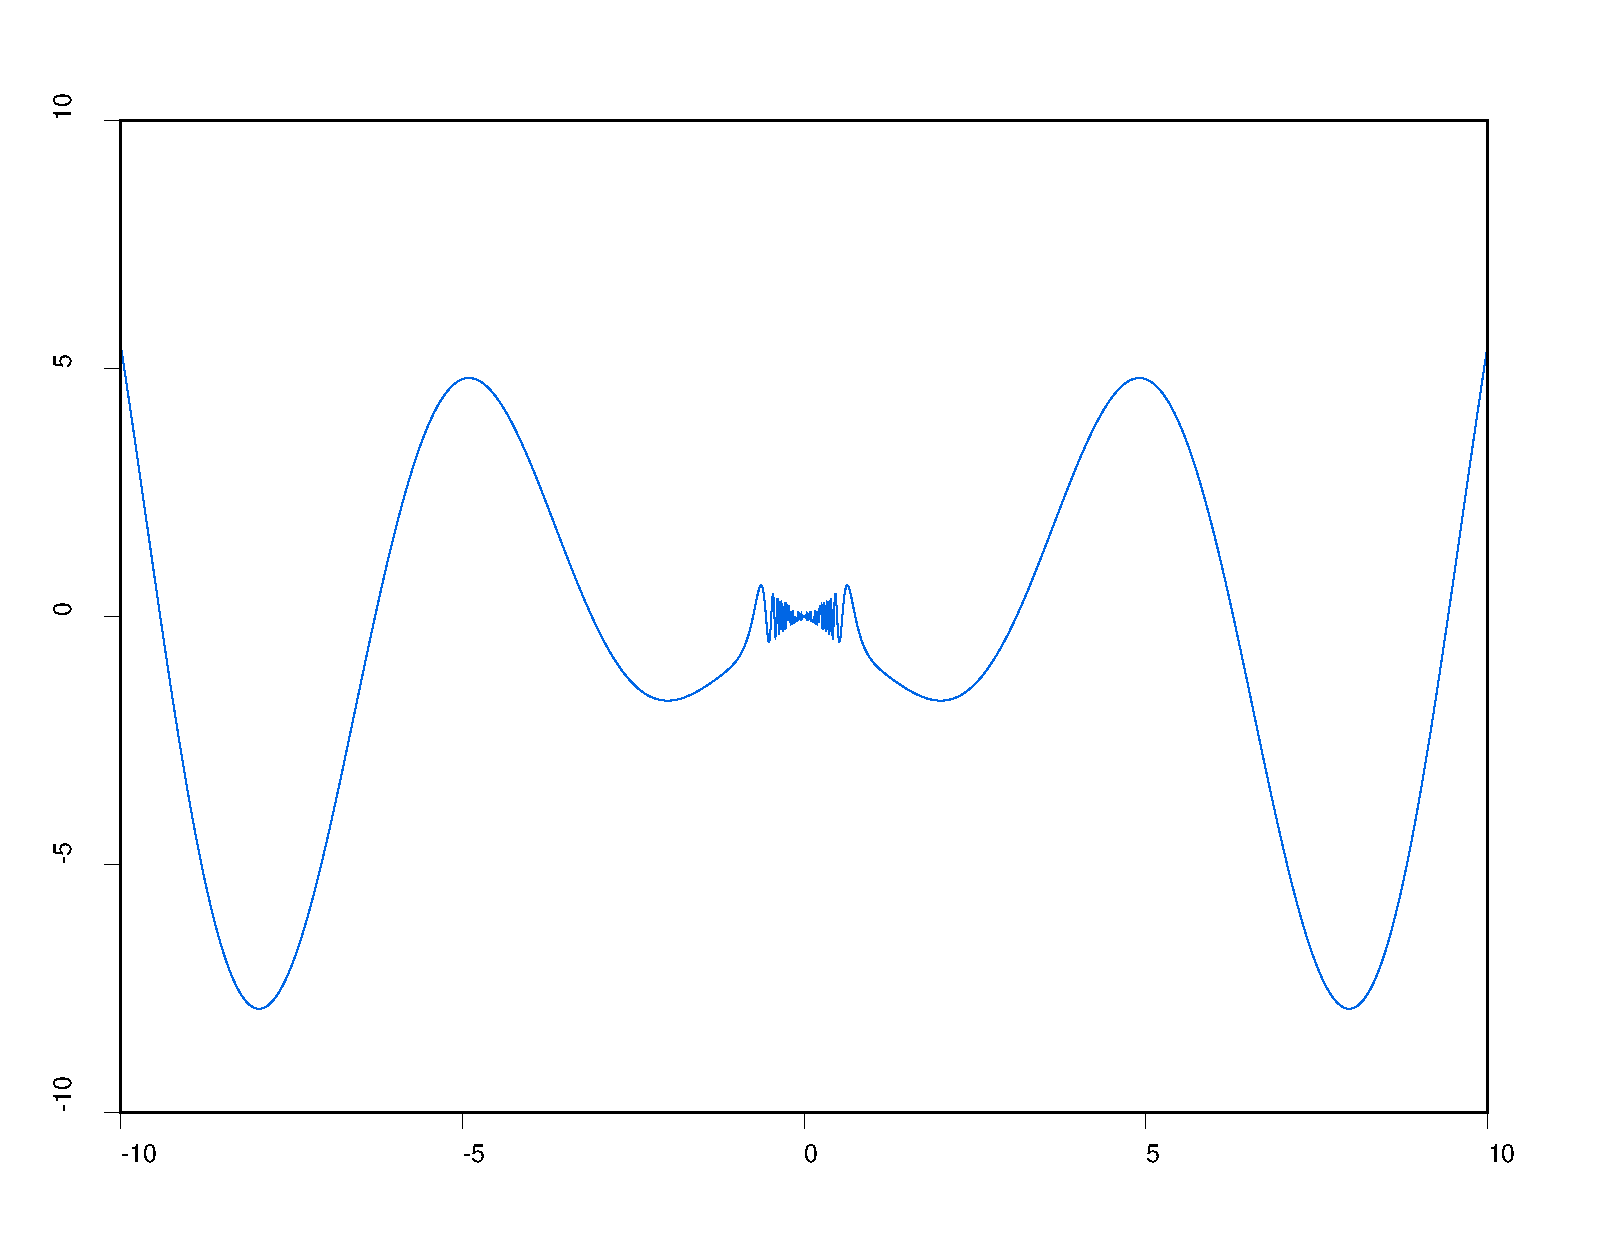
\includegraphics[width=13cm]{figures/test1.eps}
	\caption{výsledek příkazu, graf funkce $\sin \left(x + 1/x^3 \right) * -x$}
\end{figure}
\clearpage

\begin{verbatim}
./graph.exe "sin(x + 1/x^3) * -x" vystup.ps -3.4:3.4:-1.2:1.2
\end{verbatim}
Stejný příkaz, pouze použije jiný rozsah pro definiční obor ($x \in [-3, 3]$) a
obor hodnot ($y \in [-2, 2]$).
\begin{figure}[ht!]
\centering
	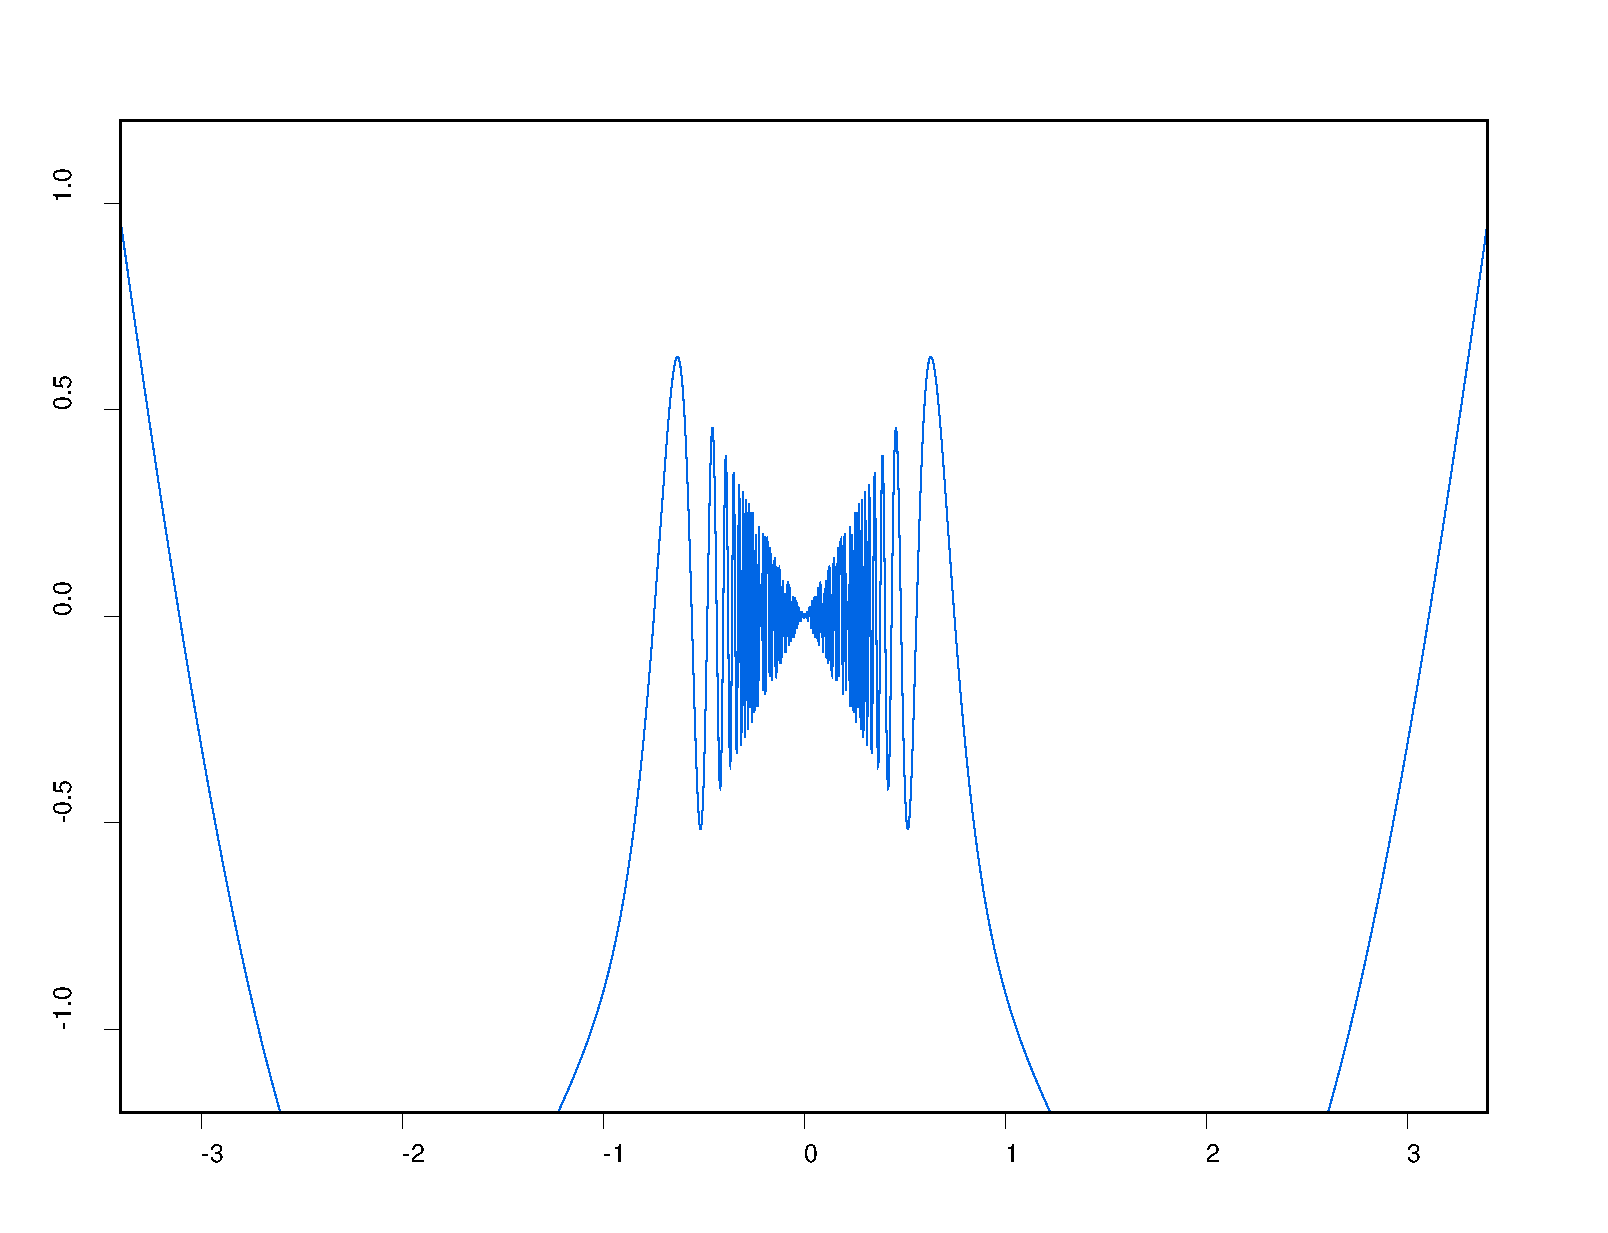
\includegraphics[width=13cm]{figures/test2.eps}
	\caption{výsledek příkazu, graf funkce $\sin \left(x + 1/x^3 \right) * -x$}
\end{figure}


Rozsahy jsou specifikovány dobrovolným parametrem, který má formát
x1:x2:y1:y2, kde x1 a y1 musí být menší než x2, respektive y2. 

Při chybném vstupu program vypíše typ chyby a ukáže na její pozici ve vstupním
řetězci. Někdy může být výpis chyby matoucí, například při chybějící závorce,
protože je chyba odhalena až na konci.

\subsection{Příklady chybného vstupu}
\begin{verbatim}
Missing parenthesis: sin(x))
                           ^
Unknown symbol: six(x)
                ^
\end{verbatim}
\begin{verbatim}
Empty subexpression: (0xdeadbeef - ())
                                    ^
\end{verbatim}
\begin{verbatim}
Missing second operand: 5 +
                          ^
\end{verbatim}
\begin{verbatim}
Number expected: -0xdeadbeef:0xbadf00d::-0xfacefeed:0xcafed00d
                                       ^
\end{verbatim}
\begin{verbatim}
Redundant: -3:3:-2:2:3
                    ^
\end{verbatim}


\section{Závěr}
Pro přehlednost byly zdrojové kódy vzhledově vyčištěny utilitou \texttt{GNU indent}~s
odsazovacím stylem Kernighan \& Ritchie a~s~volbou odstranění tabulátorů, které
v některých editorech způsobují potíže.

Největší překážkou bylo unární mínus, přestože vypadá nevinně. Použitá metoda
na parsování výrazu ho zřejmě neumí přeložit jinak, než mu dát nejvyšší
precedenci. Přesvědčila mě o tom i skutečnost, že výrobci kalkulátorů a
software používající shunting yard algoritmus na vyhodnocování aritmetických
výrazů používají právě toto řešení \cite{minus}. Možným vylepšením by bylo
použít sofistikovanější parsování převedením na strom (arithmetic tree
notation), nicměně tento způsob vypadá komplikovaně, co se týče správného
zacházení s precedencemi operátorů. Tato metoda by byla náročnější na paměť,
což může být v prostředí s omezenou pamětí (kapesní kalkulátor) kritické.

Testování proběhlo pro velké množství správných i chybných případů, všechny
dopadly úspěšně. Je zajištěno, aby nedocházelo k únikům paměti, přestože
paměťová náročnost programu je minimální a dealokování celého bloku operačním
systémem by bylo efektivnější.  Stejně jako v každém softwaru, i zde se můžou
objevit drobné chyby, prakticky nelze zajistit, aby byl program perfektní.

Snažil jsem se splnit zadání kompletně. Vygenerované grafy
jsou esteticky hezké a díky použitým metodám i prostorově úsporné. Vzhled grafu
a rámečku je inspirovaný grafy vygenerovanými programem \texttt{GNU R}, který je často
ceněn právě pro široký výběr, přehlednost a vzhled svých grafů. 

\subsection{Měření}
Paměťová náročnost je lineární v délce vstupního řetězce. Při měření programem
\texttt{valgrind} byla naměřeno využití heapu zhruba od 1~KB do 6~KB podle délky
funkce, což je přijatelné.

Časová náročnost je zcela minimální, i poměrně dlouhé funkce jsou vyhodnoceny
během zlomku vteřiny. Uživatel nepocítí žádné zpoždění.



\begin{thebibliography}{1}
\bibitem[1]{wikiShunting}
{\em Wikipedia contributors} \\ 
{\bf "Shunting-yard algorithm," Wikipedia, The Free Encyclopedia} \\
\url{http://en.wikipedia.org/w/index.php?title=Shunting-yard_algorithm&oldid=464122750} \\
(accessed December 29, 2011). \\

\bibitem[2]{shewchuk}
{\em Jonathan Shewchuk} \\
{\bf CS 61B Lecture 37: Expression Parsing} (video) 2006 \\
\url{http://www.youtube.com/watch?v=ch7fivnW45Q} \\

\bibitem[3]{minus}
{\em Douglas P. McNutt} \\
{\bf Precedence and Prophylactic Parentheses} \\
\url{http://www.macnauchtan.com/pub/precedence.html} \\
\end{thebibliography}
\end{document}
